\documentclass[11pt]{report}
\usepackage{fullpage}
%\usepackage{sourcesanspro, sourcecodepro}
\usepackage{minted}
\usepackage{graphicx}
\usepackage{awesomebox}
\usepackage{hyperref}
\usepackage{float} % stops images from moving around
\usepackage[a4paper, total={6in, 8in}, margin=0.75in]{geometry}
\usepackage{etoolbox}
\makeatletter
\patchcmd{\chapter}{\if@openright\cleardoublepage\else\clearpage\fi}{}{}{}
\RequirePackage[T1]{fontenc}
\RequirePackage[default,light,black]{roboto}

\hypersetup{
    colorlinks=true,
    linkcolor=blue,
    citecolor=blue,
    filecolor=blue,
    urlcolor=blue,
    pdfborder={0 0 0}
}

\graphicspath{{./images/}}

\title{APSC 258: Lab 4 Manual}
\author{Andre Cox \\ Scott Halston}

\begin{document}
\maketitle
\tableofcontents

\clearpage

\chapter{Introduction}
In this lab, we will be creating a simple neural network to predict the steering angle of the car.
By the end of this lab, you should have a network that can drive the car and follow the lane lines. Some parts about making the neural network are out of the scope of this course so we will provide you with a starting point for your work. You can download the code for this lab from the 
\href{https://github.com/PiCarV/Demos}{Github Repository}.

\section{Understanding Dense Layers}
Dense layers are the most basic type of neural network layer. They are simply a layer of neurons that are connected to each other. The neurons in a dense layer are simply a weighted sum of the inputs. The weights are adjusted until the network is able to predict the correct output. The process of updating the weights is called backpropagation. Generally the more neurons and layers you have the more accurate the network will be. 

\section{Gradient}
We can train our neural network using our computers; however, this will probably be slow depending on how powerful your computer is. To solve this hardware bottleneck, we will use a service called \href{https://www.gradient.run/}{Gradient}. This service provides a cloud-based platform for training neural networks and it is free for basic use. You will need to create a free account at the link above in order to be able to train your own neural network.

\section{Data}
We will be using 2 datasets. The first is a training dataset that we will use to train our neural network. The second is a test dataset that we will use to test our neural network. You can download the datasets from the link below. These files are compressed using 7zip. Do not extract this compressed file because our provided code will extract the files for you. We will show you how to do this in the next section.

%bold text
\textbf{REMEMBER TO PUT THE URL HERE}

\pagebreak

\chapter{Dense Layers Deep Dive}
\section{How dense layers work in practice}
Dense layers are a array of weights that are placed side by side. Multiple layers of dense layers can be connected together by connecting each weight in the previous layer to the weight in the next layer. This may look something like this:
% insert figure

    \begin{figure}[h]
        \begin{center}
        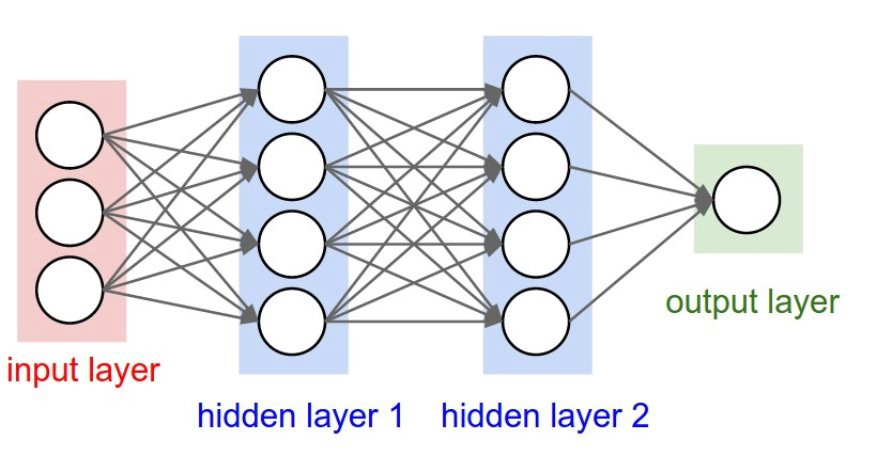
\includegraphics[width=0.5\textwidth]{denselayers.jpeg}
        \caption{Dense layers visualization}
        \label{fig:dense_layers}
        \end{center}
    \end{figure}

The weights in each neuron in the dense layer are activated by the inputs. The activation of the neuron is the weighted sum of the inputs. The activation of the neuron is then passed through a non-linear activation function to get the output. The output of the neuron is then connected to the next layer. There are many different activation functions that can be used. A couple of common ones are displayed below.

\begin{figure}
    \begin{center}
    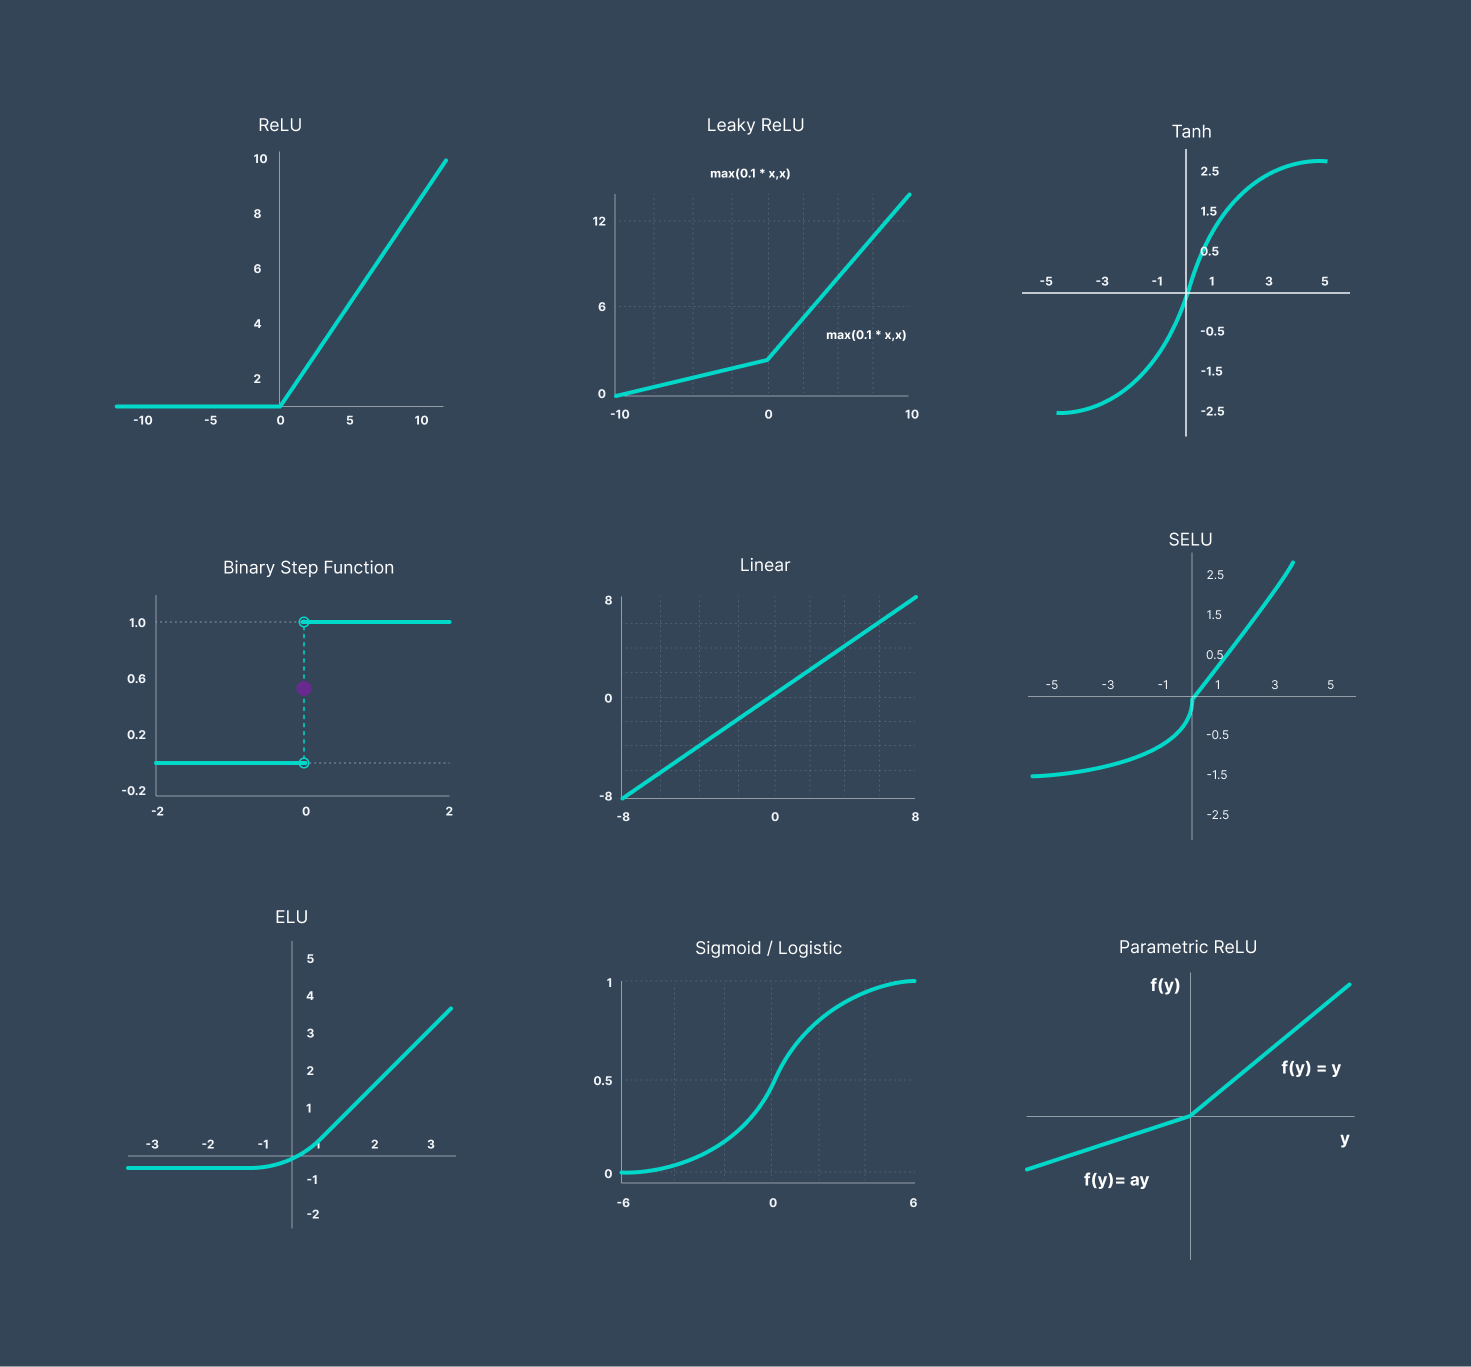
\includegraphics[width=1\textwidth]{activation functions.png}
    \caption{Common activation functions}
    \label{fig:activation_functions}
    \end{center}
\end{figure}

\section{Using Dense Layers in Keras}
Keras is the Python library that we will use to create our neural network. Keras is a high level library that allows us to create neural networks in a simple and easy way. Later you will see that we provide a pre made template for you to use. However you still need to understand how to create a neural network in Keras.

\pagebreak





\chapter{Start of the Lab}
First, we will download the demo code from the \href{https://github.com/PiCarV/Demos/archive/refs/heads/main.zip}{Github Repository}.
and then extract the files to a folder. Next, go to the folder called {PUT DIRECTORY HERE}.

\begin{minted}[breaklines=true, fontsize=\small]{bash} 
Lab Code/Lab Part 4/
\end{minted}

\begin{center}
    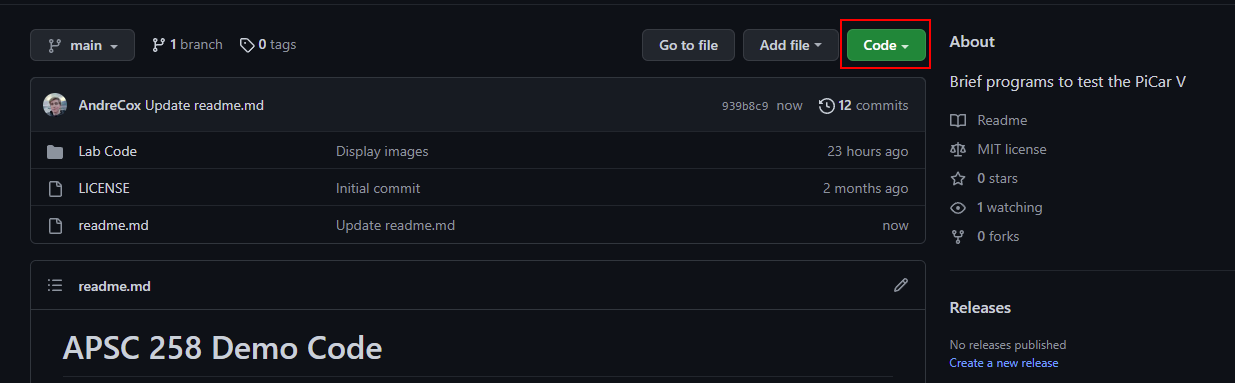
\includegraphics[scale=0.7]{github.png} 
\end{center}



Here you will find a file called “model.ipynb.” This is the file that we will use to train our neural network. In order to run this file, we will first need to upload it to Paperspace Gradient.
To do this, first, go to the Gradient website and sign up.

\begin{center}
    
\includegraphics[scale=0.6]{signinup.png}
\end{center}

Once signed up, click "CREATE A PROJECT".

\begin{center}
    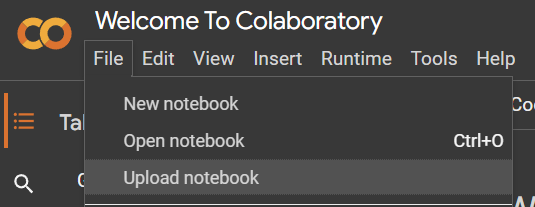
\includegraphics[scale=0.5]{creataproject.png}
\end{center}

You will be asked to choose a name for your project and you can pick whatever you want.

\begin{center}
    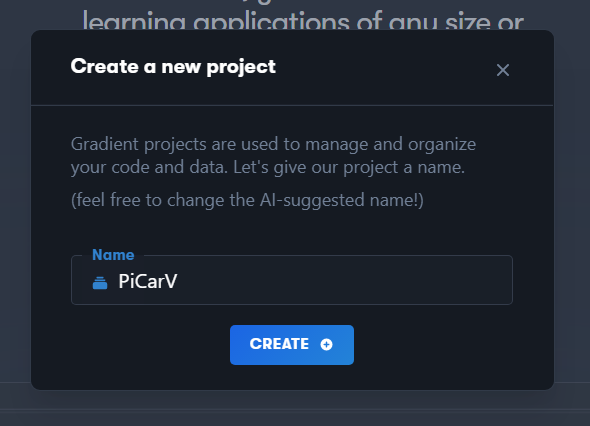
\includegraphics[scale=0.6]{nameproject.png}
\end{center}

Following the creation of your project, click "CREATE" under the Notebooks tab.

\begin{center}
    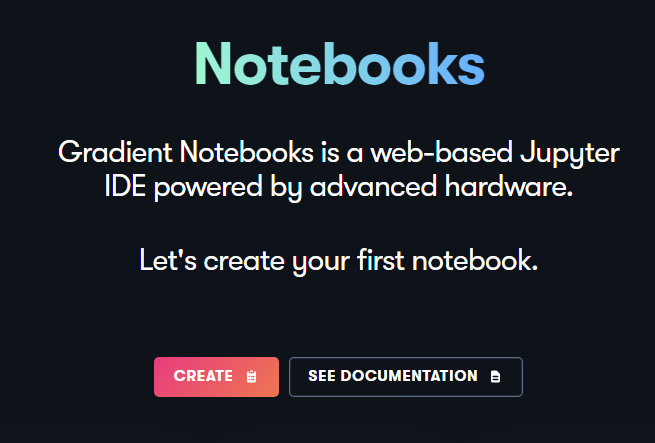
\includegraphics[scale=0.5]{notebook.png}
\end{center}

Choose "TensorFlow" as your runtime and change the “Auto-shutdown timeout” to 6 hours. This should be more than enough time to train your neural network. Once you have the correct settings selected, click "START NOTEBOOK". 

\begin{center}
    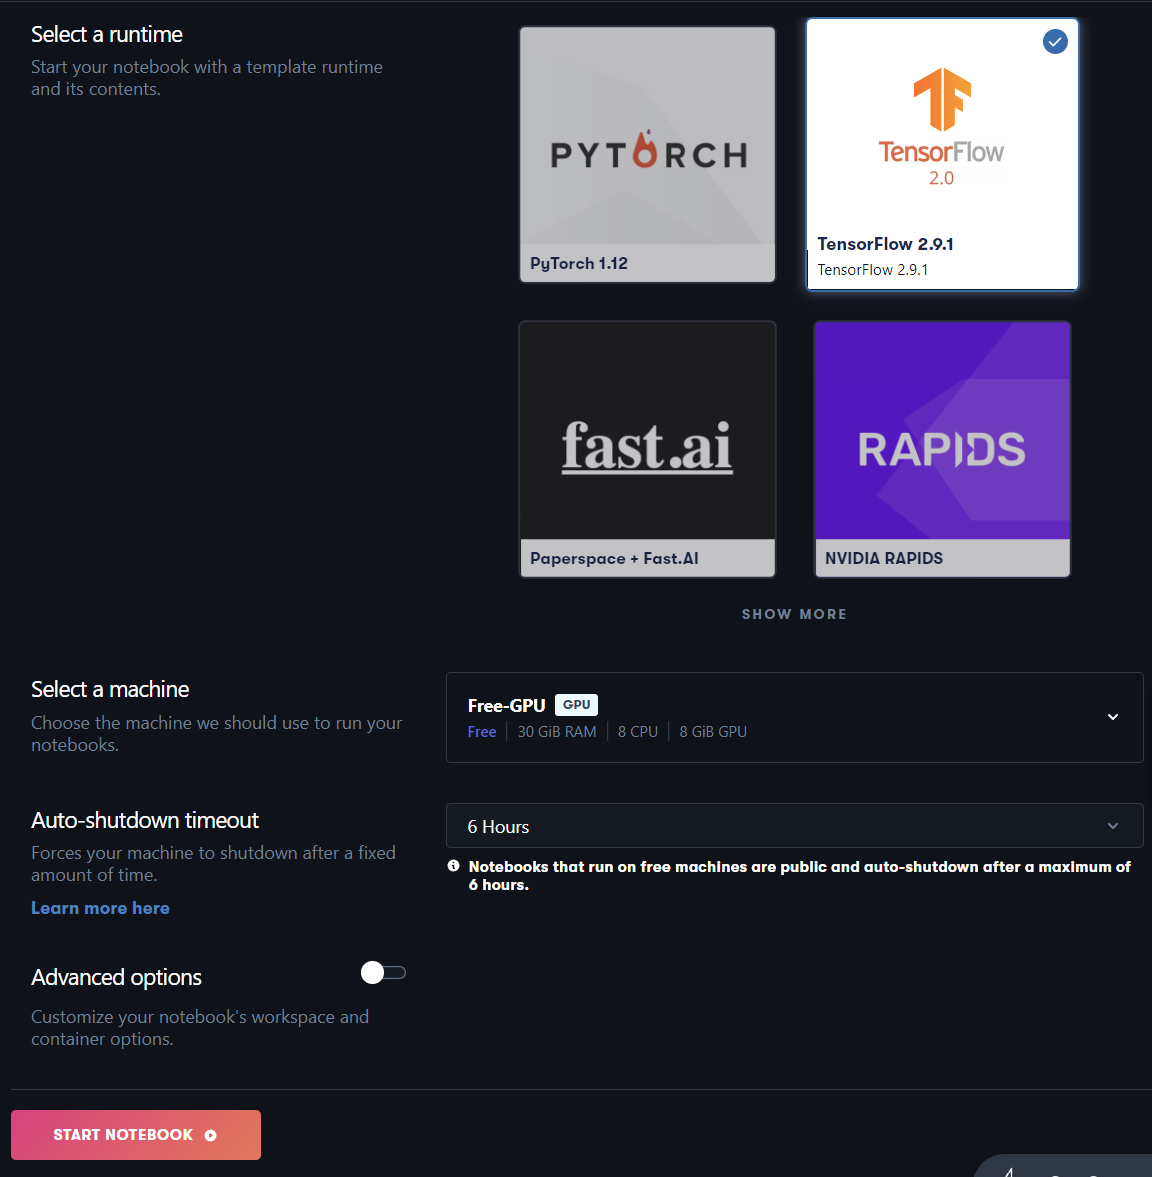
\includegraphics[scale=0.45]{settings.png}
\end{center}

After the notebook has been started, go to the left-hand side of the page and click the icon of the file. Then click the upload files icon. This is where you should upload the model.ipynb file. Once uploaded, you can open the provided model. 

\begin{center}
    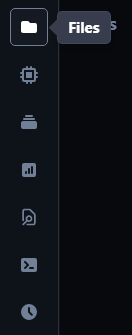
\includegraphics[scale=0.7]{files.png}
    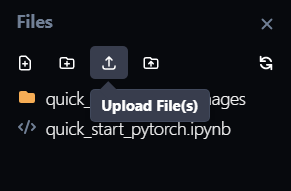
\includegraphics[scale=0.7]{uploadfiles.png}
\end{center}

\section{Data Upload}
Now we will upload the training and test datasets to Paperspace Gradient. Simply upload the data.7z file to the project the same way you uploaded the model.ipynb file.

\chapter{Running the Code}
Now that Gradient is set up and your data is uploaded you can run the code. Simply open the model.ipynb file and then run each code block one by one; make sure to wait for the previous code blocks to finish before running the next.

\section{Building your network}
Once you get to Part 4 of the code, you are ready to build your neural network. You can modify the code provided to try to get a better training result. Your goal should be to have a small mean squared error (MSE) value and consistent validation accuracy. To do this you can try adding more layers, changing the activation functions, or changing the number of neurons in the hidden layers.

\pagebreak

\section{Saving the network}
After you have trained your neural network, you can save it to a file. To do this, simply run the final code block. Before you do this, we recommend changing the name of the file to something more meaningful. After this block runs you can refresh the file browser on the left-hand side of the screen and you will see a file called model.h5 or whatever you decided to name it. This is the file that the Pi Car V will use to self-drive. You can download the file by right-clicking on it and selecting Download. 

\chapter{Running the Pi Car V}
Now that you have trained your neural network you can run the Pi Car V. To do this you can open the Demos folder you downloaded in the first part of this lab and go to the folder "Lab Code/Lab Part 4/". In this folder, you will find a file called runNetwork.py. This file will run the Pi Car V. All you need to do is connect to the Pi Car V's wifi network and then put the model.h5 file in the same folder as the runNetwork.py file. Run the file by typing "python runNetwork.py". If your file is named something else you can add some command line arguments to the file. For example "python runNetwork.py --model differentModel.h5". For a full list of command line arguments, you can type "python runNetwork.py --help".

\section{Control the Pi Car V}
Once the “runNetwork” file is running, a window will open. You can use this window to adjust the speed of the car and the colour mask.

\section{Finishing Up}
To complete this lab, you will need to experiment to get your car to follow the lane lines. This will be a bit tricky and it is okay if it is not perfect. Next lab we will introduce a new layer type that will help you achieve a better neural network.

\end{document}